\documentclass[11pt]{article}

\usepackage[letterpaper,margin=1in]{geometry}
\usepackage{amsmath}
\usepackage{booktabs}
\usepackage{longtable}
\usepackage{array}
\usepackage{graphicx}
\usepackage{float}
\usepackage{caption}
\usepackage{subcaption}
\usepackage{xcolor}
\usepackage{listings}
\usepackage{fancyhdr}
\usepackage{parskip}
\usepackage[colorlinks=true,linkcolor=blue,urlcolor=blue,citecolor=blue]{hyperref}

\definecolor{navy}{RGB}{31,58,95}
\definecolor{accentblue}{RGB}{47,110,183}
\definecolor{lightgray}{RGB}{240,240,245}

\pagestyle{fancy}
\fancyhf{}
\renewcommand{\headrulewidth}{0.4pt}
\fancyhead[R]{\small\itshape NLP GROUP ASSIGNMENT 1 \textbullet\ QUESTION 4}
\fancyfoot[C]{\small\itshape Integrated Background Editor \textbar\ Final Technical Report}

\lstset{
  breaklines=true,
  backgroundcolor=\color{black},
  basicstyle=\ttfamily\footnotesize\color{white},
  frame=none
}

\newcommand{\hcell}[2]{\begin{tabular}[b]{@{}l@{}}#1\\#2\end{tabular}}

\begin{document}

% ---------------------------------------------------------------
% Title block
% ---------------------------------------------------------------
\begin{center}
{\color{accentblue}\large\bfseries NLP GROUP ASSIGNMENT 1}\\[0.6em]
{\color{navy}\Huge\bfseries Question 4}\\[0.3em]
{\color{navy}\Huge\bfseries Integrated Background Editor}\\[1em]
{\color{accentblue}\rule{\linewidth}{1.2pt}}\\[0.8em]
{\large Live Segmentation \textbullet\ Spelling Correction \textbullet\ Constituency Parsing \textbullet\ Language-Model Grammar Checking}\\[1.5em]
\end{center}

\begin{figure}[H]
\centering
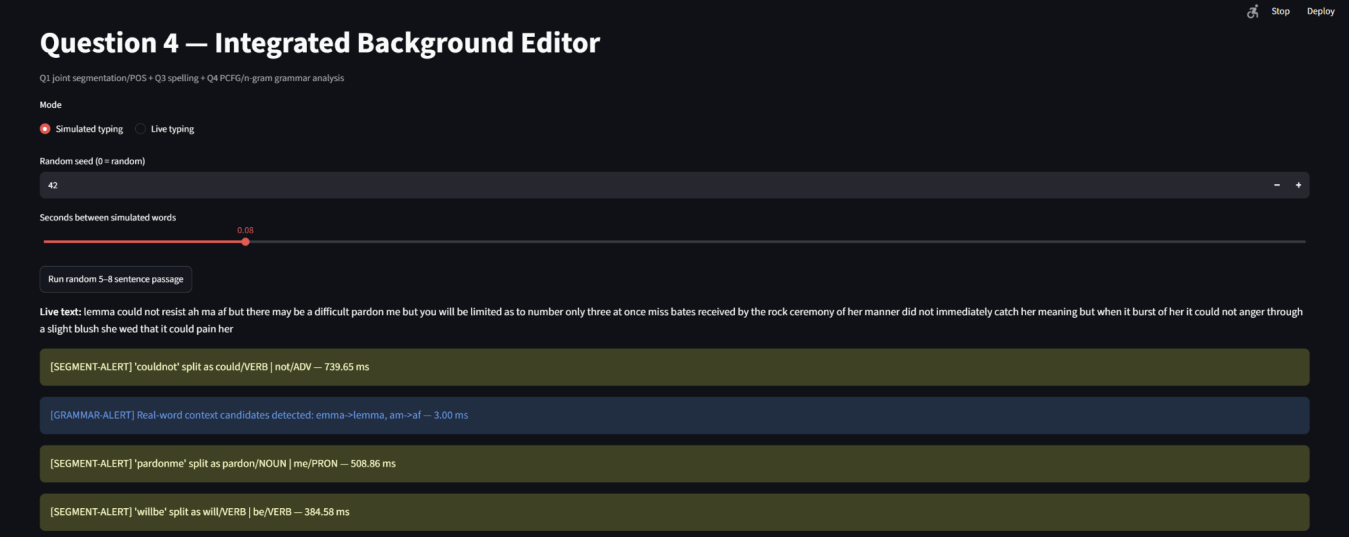
\includegraphics[width=0.92\linewidth]{assets/fig-000.png}
\caption*{\footnotesize\itshape Figure 1. Integrated Streamlit editor showing the live stream and background alerts.}
\end{figure}

\noindent
\colorbox{lightgray}{
\parbox{\linewidth}{
\textbf{\color{accentblue}Project overview} \ A single background editor processes the same incoming text stream through the trained Question 1 segmentation/POS decoder, the trained Question 3 spelling components, and a new constituency- and language-model-based grammar layer. The system supports simulated word-by-word typing and actual incremental live typing.
}}

\begin{center}
{\Large\bfseries Final Technical Report}\\[0.5em]
Q4 parameters: p = 0.08 \quad\textbullet\quad N = 10 \quad\textbullet\quad add-k = 0.1 \quad\textbullet\quad beam width = 5\\[2em]
\textbf{Group 21:} Krishna Jhanwar (12341250), Siddharth Rai (12342050), Slok Tulsyan (12342080), Vasu Garg (12342330), Gaurav Kumar (12340790)\\[0.5em]
September 8, 2026
\end{center}

\newpage

% ---------------------------------------------------------------
\section{System Overview}

The implementation is one integrated background editor rather than three independent demonstrations. Each arriving token first passes through suspicious/OOV detection. Suspicious tokens are processed by the existing Question 1 JointBeamSearchDecoder. If the decoder finds a better valid multiword segmentation, the merged token is replaced by the split words and predicted POS tags, and a SEGMENT-ALERT is emitted. Any remaining OOV word is passed to the existing Question 3 corrector and produces a SPELL-ALERT when corrected. At every N = 10 final words, the grammar layer examines the latest window using the shared language models and the Question 3-style real-word correction mechanism.

The final analysis operates on the corrected token stream, so changes made during trigger-level real-word checking are carried forward into sentence-level analysis. Sentence-level output contains PCFG parsing/log-probability, bigram and trigram log-probabilities, the selected method, a grammaticality verdict, and correction counts.

\subsection{Processing flow}

\begin{longtable}{@{}p{0.32\linewidth}p{0.60\linewidth}@{}}
\toprule
\textbf{Stage} & \textbf{Operation} \\
\midrule
\endhead
Incoming token & Read the next word/delimited token from the stream. \\
Suspicious-token check & Flag OOV or unusually long tokens. \\
Q1 joint segmentation + POS & Decode a valid split using the trained English trigram, feature model, beam width and word-length constraint. \\
Q3 spelling & For a remaining OOV word, generate candidates and choose the highest-unigram-frequency candidate. \\
Every 10 words & Run n-gram grammar plausibility and Q3-style real-word contextual checking on the latest window. \\
Final sentence analysis & Reconstruct sentences and score them with PCFG, bigram and trigram models. \\
\bottomrule
\end{longtable}

\subsection{Reuse of trained components}

\begin{longtable}{@{}p{0.16\linewidth}p{0.46\linewidth}p{0.30\linewidth}@{}}
\toprule
\textbf{Source} & \textbf{Components used} & \textbf{Q4 treatment} \\
\midrule
\endhead
Question 1 & English trigram language model and trained joint segmentation + feature-based POS decoder & Reused; no Q1 retraining in Q4 \\
Question 3 & Vocabulary/frequency data, candidate generation, spelling correction and local bigram real-word logic & Reused; no Q3 retraining in Q4 \\
Q4 & Treebank PCFG, Brown add-k bigram, integration, live editor and final analysis & Implemented for the integrated editor \\
\bottomrule
\end{longtable}

\section{Parameters and Experimental Setup}

\begin{longtable}{@{}p{0.24\linewidth}p{0.18\linewidth}p{0.50\linewidth}@{}}
\toprule
\textbf{Parameter} & \textbf{Value} & \textbf{Role} \\
\midrule
\endhead
Merge probability p & 0.08 & Creates merged-token opportunities during simulated typing. \\
Grammar trigger N & 10 words & Runs grammar/real-word checking at a fixed word-count cadence. \\
Q1 maximum word length & 20 & Same Q1 decoder constraint used by Q4. \\
Q1 beam width & 5 & Same trained Q1 decoding configuration. \\
Q1 $\alpha$, $\beta$ & 1.0, 1.0 & Same Q1 scoring weights. \\
Q4 add-k & 0.1 & Smoothing for the Brown-corpus bigram model. \\
Q3 candidate ranking & Highest unigram frequency & Selects the most frequent candidate among generated alternatives. \\
Real-word margin & 1.5 & Q3-style local bigram contextual correction threshold. \\
PCFG corpus & Penn Treebank & NLTK Treebank grammar induction. \\
LM corpus & Brown & Corpus used for the Q4 smoothed bigram. \\
Shared trigram & Q1 trained English trigram & Reused as the single shared trigram; no duplicate retraining. \\
\bottomrule
\end{longtable}

For simulated typing, the system first selects a source document/file and then samples 5--8 contiguous sentences within that source. A random seed is available for reproducible debugging. Words are streamed with a configurable sleep interval, while p = 0.08 controls removal of spaces between adjacent words.

\section{Part 1 --- Background Typing Simulation and Alerts}

The alert order is deliberately sequential. SEGMENT-ALERT has priority for OOV or unusually long tokens; SPELL-ALERT handles an OOV word that remains after segmentation; GRAMMAR-ALERT runs every 10 final words. Real-word contextual corrections are also reported as GRAMMAR-ALERT, as required by the specification.

\begin{longtable}{@{}p{0.18\linewidth}p{0.20\linewidth}p{0.52\linewidth}@{}}
\toprule
\textbf{Alert} & \textbf{Trigger} & \textbf{Action} \\
\midrule
\endhead
SEGMENT-ALERT & OOV / unusually long & Run Q1 joint beam decoder and accept a better valid multiword split with POS tags. \\
SPELL-ALERT & Still OOV & Run Q3 candidate generation and choose the highest-unigram-frequency candidate. \\
GRAMMAR-ALERT & Every 10 final words & Check the latest 10 words with n-gram plausibility and Q3-style real-word context. \\
\bottomrule
\end{longtable}

\subsection{Demonstrated Run A --- seed 42}

The following table reproduces the observed alert transcript in structured form.

\begin{longtable}{@{}p{0.16\linewidth}p{0.20\linewidth}p{0.38\linewidth}p{0.13\linewidth}@{}}
\toprule
\textbf{Alert type} & \textbf{Observed token(s)} & \textbf{Action / correction} & \textbf{Latency (ms)} \\
\midrule
\endhead
SEGMENT-ALERT & couldnot & could/VERB \textbar\ not/ADV & 342.75 \\
GRAMMAR-ALERT & emma, am & emma$\rightarrow$lemma, am$\rightarrow$af & 2.11 \\
SEGMENT-ALERT & willbe & will/VERB \textbar\ be/VERB & 276.02 \\
SEGMENT-ALERT & limitedas & limited/VERB \textbar\ as/ADP & 354.97 \\
GRAMMAR-ALERT & bea, difficulty, as & bea$\rightarrow$be, difficulty$\rightarrow$difficult, as$\rightarrow$af & 1.97 \\
SEGMENT-ALERT & atonce & at/ADP \textbar\ once/ADV & 292.20 \\
GRAMMAR-ALERT & deceived & deceived$\rightarrow$received & 3.13 \\
SEGMENT-ALERT & hermanner & her/DET \textbar\ manner/NOUN & 392.25 \\
SEGMENT-ALERT & didnot & did/VERB \textbar\ not/ADV & 221.83 \\
GRAMMAR-ALERT & mock, catch & mock$\rightarrow$rock, catch$\rightarrow$watch & 3.18 \\
GRAMMAR-ALERT & her, on & her$\rightarrow$he, on$\rightarrow$of & 3.08 \\
SEGMENT-ALERT & angerthough & anger/ADV \textbar\ though/ADP & 369.93 \\
SEGMENT-ALERT & shewed & she/PRON \textbar\ wed/VERB & 328.68 \\
GRAMMAR-ALERT & though & though$\rightarrow$through & 3.26 \\
\bottomrule
\end{longtable}

\noindent Run summary: 63 final tokens, 8 segmentation merges, 6 grammar triggers, average token-stage latency 46.90 ms, average grammar-trigger latency 2.79 ms, and 0 non-word SPELL-ALERT corrections.

\subsection{Demonstrated Run B --- seed 123}

\begin{longtable}{@{}p{0.18\linewidth}p{0.20\linewidth}p{0.36\linewidth}p{0.12\linewidth}@{}}
\toprule
\textbf{Alert type} & \textbf{Observed token(s)} & \textbf{Action / correction} & \textbf{Latency (ms)} \\
\midrule
\endhead
SEGMENT-ALERT & youtalk & you/PRON \textbar\ talk/VERB & 358.00 \\
SEGMENT-ALERT & whisperedturnbull & whispered/VERB \textbar\ turn/NOUN \textbar\ bull/NOUN & 914.22 \\
GRAMMAR-ALERT & bull & bull$\rightarrow$ball & 4.52 \\
SEGMENT-ALERT & thewall & the/DET \textbar\ wall/NOUN & 332.80 \\
SEGMENT-ALERT & macian & ma/DET \textbar\ c/. \textbar\ i/. \textbar\ an/DET & 264.54 \\
SEGMENT-ALERT & thecabman & the/DET \textbar\ cab/NOUN \textbar\ man/NOUN & 479.78 \\
GRAMMAR-ALERT & ma, i, an, cab & ma$\rightarrow$a, i$\rightarrow$is, an$\rightarrow$as, cab$\rightarrow$car & 1.74 \\
SEGMENT-ALERT & scotchdrawl & s/. \textbar\ c/. \textbar\ o/. \textbar\ t/. \textbar\ c/. \textbar\ h/. \textbar\ drawl/NOUN & 500.81 \\
GRAMMAR-ALERT & o, t, drawl & o$\rightarrow$of, t$\rightarrow$a, drawl$\rightarrow$draw & 2.08 \\
SEGMENT-ALERT & st & s/. \textbar\ t/. & 36.27 \\
GRAMMAR-ALERT & us, s, t & us$\rightarrow$is, s$\rightarrow$a, t$\rightarrow$it & 3.56 \\
SEGMENT-ALERT & pancras & pan/VERB \textbar\ c/. \textbar\ r/. \textbar\ as/ADP & 234.77 \\
SEGMENT-ALERT & verra & v/. \textbar\ err/NOUN \textbar\ a/DET & 139.90 \\
GRAMMAR-ALERT & pan, r, as & pan$\rightarrow$an, r$\rightarrow$or, as$\rightarrow$a & 1.85 \\
SEGMENT-ALERT & cabman & cab/NOUN \textbar\ man/NOUN & 264.50 \\
SEGMENT-ALERT & dlike & d/. \textbar\ like/ADP & 186.48 \\
GRAMMAR-ALERT & cab, d & cab$\rightarrow$car, d$\rightarrow$do & 1.57 \\
SEGMENT-ALERT & arst & a/DET \textbar\ r/. \textbar\ s/. \textbar\ t/. & 91.51 \\
SEGMENT-ALERT & asecond & a/DET \textbar\ second/ADJ & 259.07 \\
GRAMMAR-ALERT & s, t & s$\rightarrow$a, t$\rightarrow$to & 2.23 \\
SEGMENT-ALERT & macianheard & ma/DET \textbar\ c/. \textbar\ i/. \textbar\ an/DET \textbar\ heard/NOUN & 423.04 \\
GRAMMAR-ALERT & i & i$\rightarrow$is & 1.27 \\
GRAMMAR-ALERT & on & on$\rightarrow$in & 2.07 \\
SEGMENT-ALERT & getover & get/VERB \textbar\ over/PRT & 241.64 \\
\bottomrule
\end{longtable}

\noindent Run summary: 119 final tokens, 15 segmentation merges, 10 grammar triggers, average token-stage latency 54.35 ms, average grammar-trigger latency 2.37 ms, and all 5 final sentences parsed by the PCFG.

\section{Streamlit Live Deployment}

The Streamlit application exposes both simulated typing and actual incremental live typing. In live mode, the committed prefix is processed as the user types; the unfinished final token is retained until a delimiter is entered. The interface displays the processed stream, alerts, live latency, grammar-trigger count, and final analysis.

\begin{figure}[H]
\centering
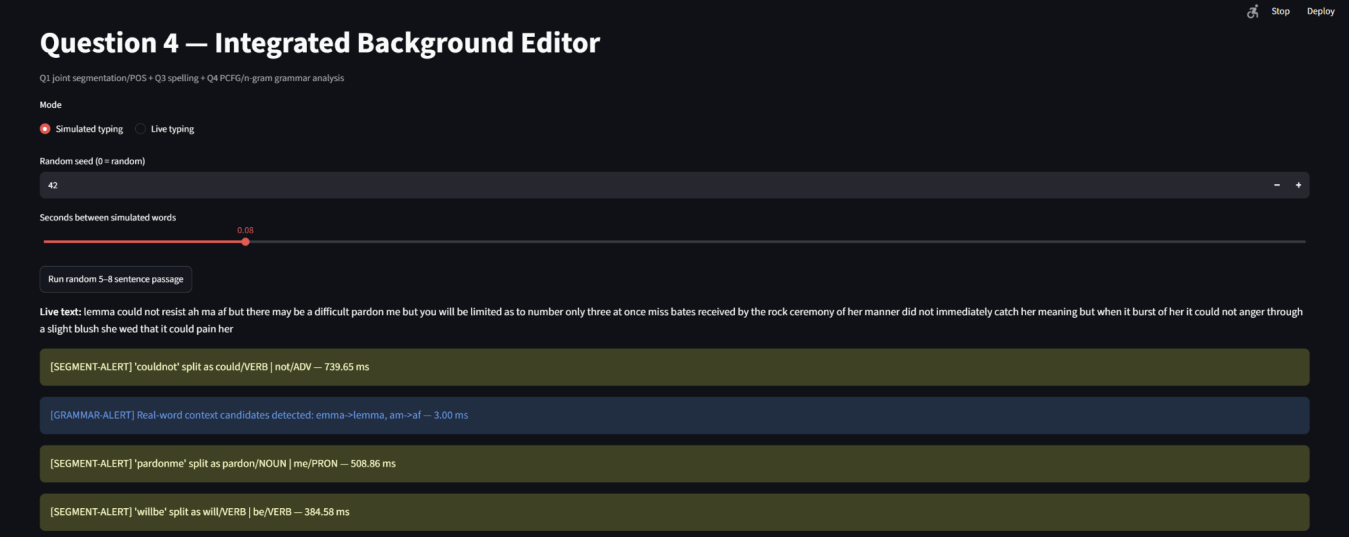
\includegraphics[width=0.92\linewidth]{assets/fig-000.png}
\caption*{\footnotesize\itshape Figure 2. Streamlit integrated editor: simulated mode with the live stream and multiple background alerts.}
\end{figure}

\begin{figure}[H]
\centering
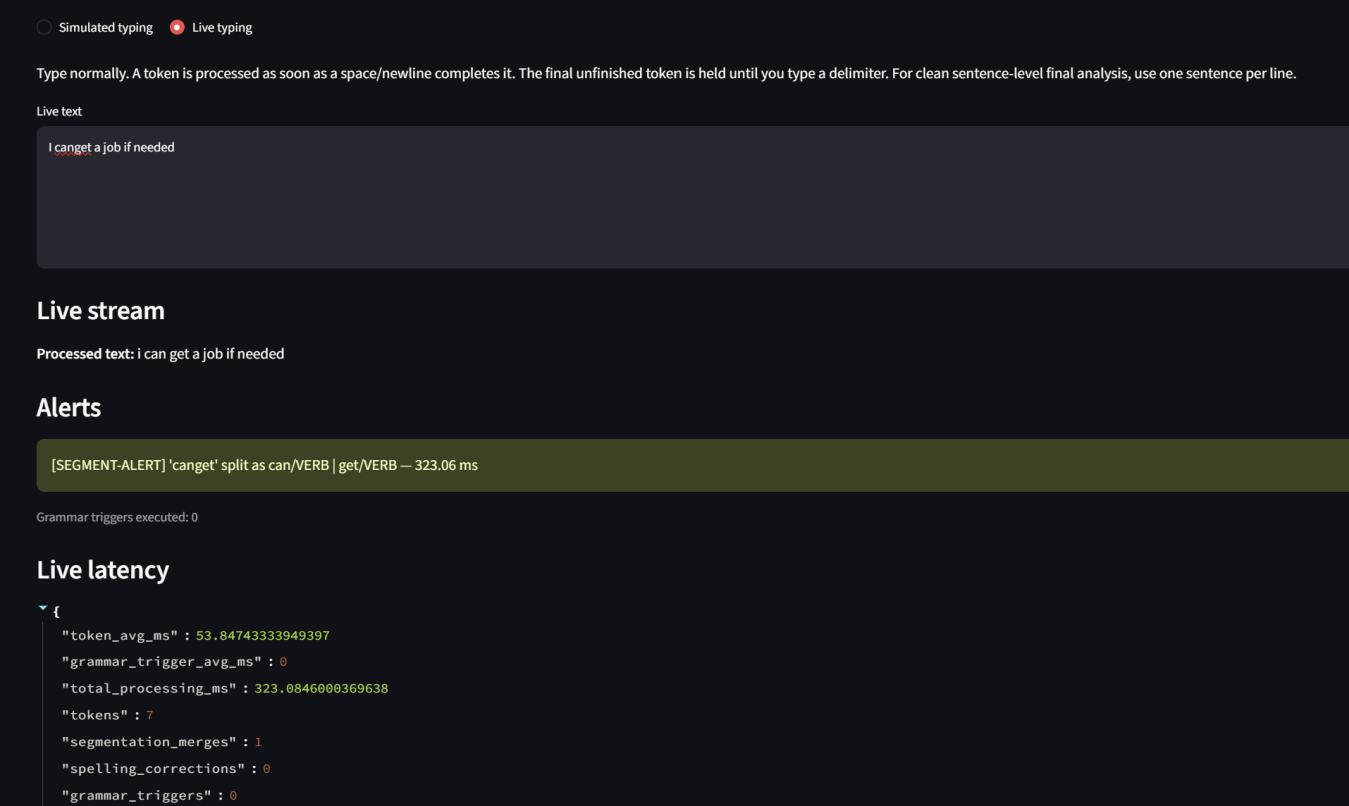
\includegraphics[width=0.92\linewidth]{assets/fig-002.png}
\caption*{\footnotesize\itshape Figure 3. Actual incremental live-typing mode showing an immediate segmentation alert and live latency statistics.}
\end{figure}

The screenshots show the editor operating as one integrated interface: a token can be processed by Q1, the resulting stream can be checked by the grammar layer, and the same corrected stream can then be used for sentence-level analysis.

\section{Part 2 --- PCFG Constituency Parser}

A probabilistic context-free grammar is induced from the NLTK Penn Treebank sample. The parser indexes binary, unary and lexical productions and performs a custom Viterbi CKY-style dynamic program with unary closure. If no complete parse can be constructed, the result is reported as UNPARSEABLE rather than causing the application to fail.

\subsection{POS tagset reconciliation}

The Question 1 English feature-based POS model uses Brown/Universal-style tags, whereas Treebank lexical productions use Penn Treebank tags. A deterministic mapping is therefore applied before PCFG parsing. The mapping includes cases such as PRT $\rightarrow$ RP and normalization across the verb family, with conservative fallback handling for robustness.

No independent numerical tag-mapping accuracy experiment was performed; therefore the report does not claim a measured accuracy loss from the mapping. A known limitation is that compact mappings can collapse distinctions represented more finely in PTB.

\section{Part 3 --- Smoothed N-gram Language Models}

The Q4 grammar layer uses a Brown-corpus add-k smoothed bigram with k = 0.1 and reuses the trained English Q1 trigram as the single shared trigram. The Q1 trigram remains the model used by the segmentation scorer, while the trained Q3 bigram remains the model used by the real-word correction component. Q4 does not retrain the Q1 or Q3 models.

For a bigram, add-k smoothing assigns a non-zero probability by adding k to the observed count and kV to the denominator. The trigram layer is reused from Q1 as the shared trained English trigram. Sentence scores are accumulated as log-probabilities; the implementation's average log-probability is equivalent to the logarithmic form of perplexity, so lower average log-probability corresponds to lower model plausibility.

\noindent
\colorbox{lightgray}{
\parbox{\linewidth}{
\textbf{\color{accentblue}Model-sharing design} \ The shared-trigram choice avoids duplicate retraining while preserving the already-trained Q1 English trigram required by the integrated pipeline.
}}

\section{Part 4 --- Final Passage Analysis}

After live processing, sentence boundaries are reconstructed from the final corrected stream. Each sentence is scored by the PCFG when parseable and by the shared bigram/trigram models. The selected method is reported together with a final verdict. The decision rule prefers a successful PCFG result when its normalized score is not a strong outlier; otherwise it uses the trigram when coverage is adequate and falls back to the bigram when necessary.

\subsection{Final analysis --- seed 42}

\begingroup
\scriptsize
\setlength{\tabcolsep}{3pt}
\begin{longtable}{@{}p{0.14\linewidth}p{0.135\linewidth}p{0.095\linewidth}p{0.095\linewidth}p{0.095\linewidth}p{0.09\linewidth}p{0.125\linewidth}p{0.045\linewidth}p{0.045\linewidth}@{}}
\toprule
\textbf{sentence} & \hcell{pcfg\_}{result} & \hcell{pcfg\_}{logprob} & \hcell{bigram\_}{logprob} & \hcell{trigram\_}{logprob} & \hcell{chosen\_}{method} & \textbf{verdict} & \hcell{seg.}{merges} & \hcell{spell.}{corr.} \\
\midrule
\endhead
lemma could not resist & PARSED & -67.571653 & -42.541154 & -54.102515 & PCFG & LIKELY-GRAMMATICAL & 1 & 1 \\
ah & UNPARSEABLE & NaN & -16.818304 & -23.973234 & TRIGRAM & POTENTIALLY-UNGRAMMATICAL & 0 & 0 \\
ma af but there may be difficult & UNPARSEABLE & NaN & -52.441261 & -84.789246 & TRIGRAM & POTENTIALLY-UNGRAMMATICAL & 0 & 3 \\
pardon me but you will be limited af to number only three at once & PARSED & -211.843004 & -102.943547 & -158.403700 & PCFG & LIKELY-GRAMMATICAL & 3 & 1 \\
miss bates received by the rock ceremony of her manner did not immediately watch he & PARSED & -487.729922 & -297.492240 & -402.981402 & PCFG & LIKELY-GRAMMATICAL & 4 & 6 \\
meaning but when it burst of her it could not anger through a slight blush she wed that it could pain her & & & & & & & & \\
\bottomrule
\end{longtable}
\endgroup

\subsection{Final analysis --- seed 123}

\begingroup
\scriptsize
\setlength{\tabcolsep}{3pt}
\begin{longtable}{@{}p{0.14\linewidth}p{0.135\linewidth}p{0.095\linewidth}p{0.095\linewidth}p{0.095\linewidth}p{0.09\linewidth}p{0.125\linewidth}p{0.045\linewidth}p{0.045\linewidth}@{}}
\toprule
\textbf{sentence} & \hcell{pcfg\_}{result} & \hcell{pcfg\_}{logprob} & \hcell{bigram\_}{logprob} & \hcell{trigram\_}{logprob} & \hcell{chosen\_}{method} & \textbf{verdict} & \hcell{seg.}{merges} & \hcell{spell.}{corr.} \\
\midrule
\endhead
you talk to him aminute whispered turn ball and stepped back into the shadow of the wall & PARSED & -184.849924 & -122.613490 & -178.809218 & PCFG & LIKELY-GRAMMATICAL & 3 & 1 \\
we want you said a c is as to the car man with a superb s c of a c h draw of indifference and assurance to drive is to a it an c or a station v err a quick & PARSED & -484.223880 & -316.880563 & -434.501224 & PCFG & LIKELY-GRAMMATICAL & 6 & 13 \\
very sorry sir said the car man but i do like to know it was all right & PARSED & -232.972965 & -115.887696 & -177.299774 & PCFG & LIKELY-GRAMMATICAL & 2 & 2 \\
might i a r a to where you come from sir & PARSED & -202.505878 & -99.200096 & -129.912323 & PCFG & LIKELY-GRAMMATICAL & 1 & 2 \\
a second after he spoke ma c is an heard a heavy voice in the otherside of the wall saying i suppose i d better get over and look for them & PARSED & -351.381940 & -221.452713 & -321.660615 & PCFG & LIKELY-GRAMMATICAL & 3 & 2 \\
\bottomrule
\end{longtable}
\endgroup

\begin{figure}[H]
\centering
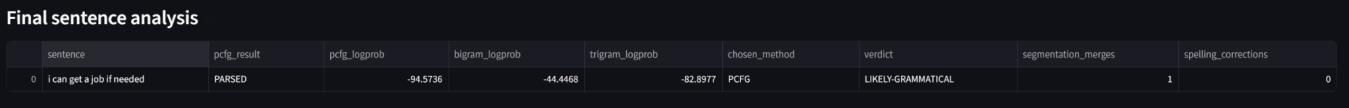
\includegraphics[width=0.92\linewidth]{assets/fig-003.png}
\caption*{\footnotesize\itshape Figure 4. Streamlit final sentence-analysis table displaying sentence-level model scores and the selected verdict.}
\end{figure}

\section{Live Latency Results}

\begin{longtable}{@{}p{0.10\linewidth}p{0.10\linewidth}p{0.12\linewidth}p{0.12\linewidth}p{0.13\linewidth}p{0.13\linewidth}p{0.15\linewidth}@{}}
\toprule
\textbf{Run} & \textbf{Final tokens} & \textbf{Segmentation merges} & \textbf{Grammar triggers} & \textbf{Token avg (ms)} & \textbf{Grammar avg (ms)} & \textbf{Total processing (ms)} \\
\midrule
\endhead
Seed 42 & 63 & 8 & 6 & 46.8977 & 2.7873 & 2596.0999 \\
Seed 123 & 119 & 15 & 10 & 54.3503 & 2.3659 & 4752.1369 \\
\bottomrule
\end{longtable}

The token-stage measurement covers per-token segmentation and spelling processing, while the grammar-trigger measurement is maintained separately. This separation makes the cost of the periodic grammar layer visible rather than mixing it with the per-token path.

\section{Speed Demon Benchmark}

The Speed Demon benchmark processes exactly 1,000 simulated words through the complete per-token segmentation + spelling path, then measures the grammar-trigger check separately. The grammar trigger is isolated so that its computational cost can be compared directly with the dominant per-token work.

\begin{longtable}{@{}p{0.55\linewidth}p{0.30\linewidth}@{}}
\toprule
\textbf{Metric} & \textbf{Measured value} \\
\midrule
\endhead
n\_words & 1000.000000 \\
full\_pipeline\_seconds & 363.785966 \\
full\_pipeline\_avg\_ms & 363.785966 \\
grammar\_only\_seconds & 0.004083 \\
grammar\_only\_avg\_ms\_per\_word & 0.004083 \\
added\_segmentation\_spelling\_seconds & 363.781883 \\
added\_segmentation\_spelling\_avg\_ms & 363.781883 \\
\bottomrule
\end{longtable}

\begin{figure}[H]
\centering
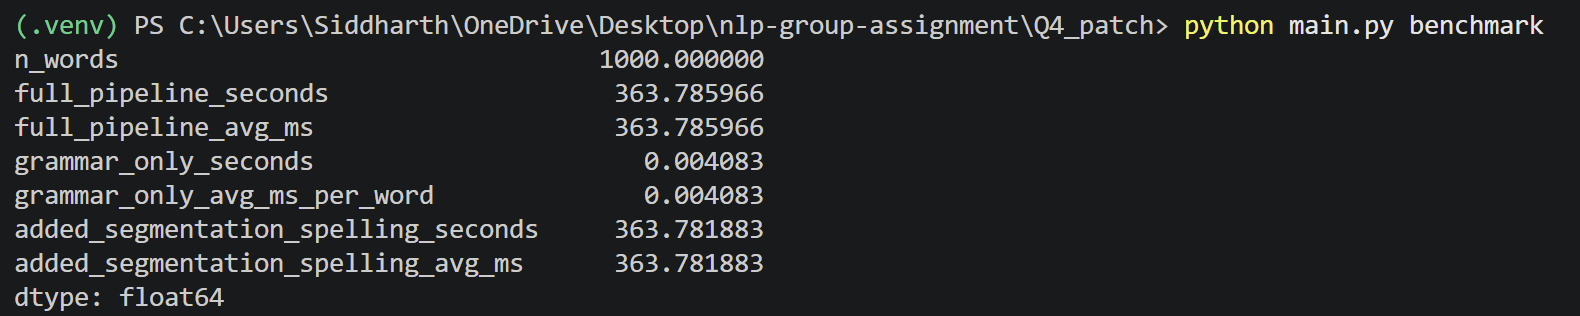
\includegraphics[width=0.92\linewidth]{assets/fig-004.png}
\caption*{\footnotesize\itshape Figure 5. Exact benchmark output for the 1,000-word Speed Demon run.}
\end{figure}

The measured full-pipeline time is 363.785966 s, or 363.785966 ms/word. The isolated grammar check requires only 0.004083 s in total, whereas segmentation + spelling accounts for 363.781883 s. Thus essentially all measured batch time comes from repeated Q1 beam decoding and the Q3 spelling path. This explains why periodic grammar checking is suitable for the live editor while the Q1 decoder is the principal computational bottleneck at machine-speed input.

\section{Comparative Analysis}

\subsection{Live alerts versus final verdict}

Exact one-to-one agreement between live alerts and the final sentence verdict is not expected. Live checks operate on individual tokens and fixed 10-word windows, whereas the final decision is sentence-level and includes constituency structure. A token can therefore receive a contextual alert even when the completed sentence is PCFG-parseable, and a parseable sentence can still contain locally suspicious word choices. The seed-123 corrections such as bull$\rightarrow$ball and cab$\rightarrow$car illustrate the possibility of false-positive local real-word corrections.

\subsection{PCFG versus n-grams}

PCFG evidence is hierarchical and structural: it asks whether the POS-tagged sentence can be generated by a Treebank-derived grammar and assigns a probabilistic parse. Bigram and trigram evidence is sequential and local: it measures the plausibility of adjacent or short-context word sequences. The two views are complementary. N-grams can provide a score even when the PCFG cannot parse a sentence, while the PCFG can represent constituency structure that local adjacency statistics do not encode.

\subsection{Effect of N and p}

Increasing p creates more merged-token opportunities and therefore increases segmentation workload and alert activity. Decreasing p produces a cleaner demonstration but exercises Q1 less often. A smaller N detects grammar/real-word issues sooner but increases trigger frequency and alert noise; a larger N reduces overhead and noise but delays detection. The chosen p = 0.08 and N = 10 provide a practical coursework setting.

\subsection{Subsystem interactions}

The pipeline is sequential. A segmentation split changes word boundaries and POS tags, which can improve PCFG coverage and alter n-gram scores. A spelling or real-word correction changes the local context and can affect later grammar checks and the final selected method. For example, the correction of couldnot into could not changes the token sequence used by downstream analysis.

\subsection{Performance implication}

The live runs show token-stage averages around 47--54 ms, while grammar-trigger averages are around 2--3 ms. The 1,000-word benchmark confirms the same architectural pattern at scale: the periodic grammar layer is inexpensive compared with repeated Q1 joint decoding and Q3 processing. For higher-throughput deployment, the natural optimization targets are Q1 decoding, caching, and controlled throttling.

\section{Observed Limitations}

This implementation is a coursework prototype and its correction behavior is intentionally tied to the supplied Q1/Q3 components. The Q3-style local real-word mechanism can produce semantically incorrect substitutions when local bigram evidence is misleading. The seed-123 run provides concrete examples. Similarly, PCFG parseability is model-relative and does not imply semantic correctness. The Speed Demon benchmark also demonstrates that repeated Q1 beam decoding is computationally expensive at machine-speed input.

\section{Conclusion}

Question 4 is implemented as a single integrated background editor combining trained Q1 segmentation/POS, trained Q3 spelling components, Treebank-based PCFG parsing, and smoothed n-gram grammar checking. The editor supports both simulated and actual incremental live typing, emits the required alert types at the specified stages, records separate latency measures, and performs sentence-level final analysis on the corrected stream.

Two independent seeded runs demonstrate repeatable integrated behavior with different sampled passages. The final sentence tables expose PCFG, bigram and trigram evidence together with the selected decision and correction counts. The 1,000-word benchmark further isolates the dominant computational cost, showing that the Q1/Q3 per-token path is substantially more expensive than the periodic grammar-trigger check.

\appendix
\section*{Appendix A --- Raw Benchmark Transcript}

\begin{lstlisting}
n_words                                1000.000000
full_pipeline_seconds                   363.785966
full_pipeline_avg_ms                    363.785966
grammar_only_seconds                      0.004083
grammar_only_avg_ms_per_word              0.004083
added_segmentation_spelling_seconds     363.781883
added_segmentation_spelling_avg_ms      363.781883
dtype: float64
\end{lstlisting}

\section*{Appendix B --- Run-level summary}

\begin{longtable}{@{}p{0.09\linewidth}p{0.10\linewidth}p{0.08\linewidth}p{0.11\linewidth}p{0.11\linewidth}p{0.11\linewidth}p{0.10\linewidth}p{0.13\linewidth}@{}}
\toprule
\textbf{Seed} & \textbf{Final tokens} & \textbf{Merges} & \textbf{Grammar triggers} & \textbf{Token avg ms} & \textbf{Grammar avg ms} & \textbf{PCFG parsed} & \textbf{Non-word SPELL-ALERT corrections} \\
\midrule
\endhead
Seed 42 & 63 & 8 & 6 & 46.8977 & 2.7873 & 4/5 & 0 \\
Seed 123 & 119 & 15 & 10 & 54.3503 & 2.3659 & 5/5 & 0 \\
\bottomrule
\end{longtable}

\end{document}
